\section{Space Dynamics/Kepler Orbits}
\f{Typical coordinate systems:}
\begin{itemize}
 \item spacecraft-fixed
 \begin{itemize}
  \item Mittelpunkt des Satelliten = Ursprung
  \item nadir = z-Achse, nominale Geschwindigkeit = x-Achse
  \item gut, um Position und Orientierung der Satelliteninstrumente festzustellen
 \end{itemize}
 \item earth-fixed 
 \begin{itemize}
  \item Mittelpunkt der Erde = Ursprung
  \item durch greenwich meridian = x-Achse
  \item Geolocation, Satellitenbewegung
 \end{itemize}
 \item roll, pitch and yaw-coordinates 
 \item celestial coordinates
 \begin{itemize}
  \item Mittelpunkt der Erde = Ursprung
  \item Richtung Frühlingspunkt = x-Achse
  \item Orbitanalyse, Astronomie
 \end{itemize}
\end{itemize}
\f{Keplergesetze}
\begin{enumerate}
 \item der Orbit eines jeden Planeten ist eine Ellipse, wobei die Sonne in einem der Fixpunkte liegt
 \item die Verbindungslinie zwischen Sonne und Planet überstreicht in gleichen Zeiten gleiche Flächen 
 \item die Quadrate der Umlaufzeiten sind proportional zu den Kuben der großen Halbachsen
\end{enumerate}
\f{Ellipsendinge}
\begin{itemize}
 \item a \dots große Halbachse
 \item $\varepsilon$, e \dots Exzentrizität, ``Abplattung'' der Ellipse ($\varepsilon$=0: Kreis, $\varepsilon$=1: Parabel, $0<\varepsilon<1$: Ellipse)
\end{itemize}
\f{Begriffe: }
\begin{itemize}
 \item Periapsis: Punkt der Ellipse, der am nähesten an dem Zentralkörper liegt (bei Sonne: Perihel, bei Erde: Perigäum)
 \item Apoapsis: Punkt der Ellipse, der am weitesten entfernt vom Zentralkörper liegt (bei Sonne: Apohel, bei Erde: Apogäum)
 \item Distanz zu Periapsis $r_p = a(1-\varepsilon)$, Distanz zu Apoapsis $r_a = a(1+\varepsilon)$
\end{itemize}
\f{6 Bahnelemente:}
\vspace*{10pt}

\begin{figure}[!ht]
\begin{minipage}{0.35\textwidth}
 \begin{itemize}
  \item große Halbachse a
  \item Exzentrizität $\varepsilon$
  \item inclination i
  \item right ascension of the ascending node $\Omega$
  \item argument of perigee $\omega$
  \item true anomaly $\nu$
 \end{itemize} 
\end{minipage}
\hfill
\begin{minipage}{0.64\textwidth}
  \centering
  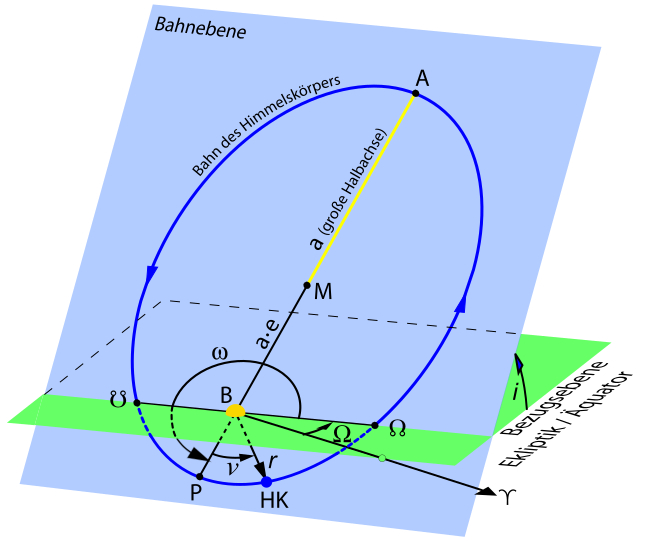
\includegraphics[scale=0.55]{BahnelementeEllipse}
\end{minipage}
\end{figure}
\noindent \f{Lieblingsformel}
\[T = 2\pi\sqrt{\frac{a^3}{\mu}}\]
\f{Change of the right ascension of the ascending node}
\[\Delta \Omega = - \frac{3\pi J_2R_E^2}{a^2(1-\varepsilon^2)^2}cos(i)\]
\f{Change of the argument of perigee}
\[\Delta \omega = \frac{3\pi J_2R_E^2}{2a^2(1-\varepsilon^2)^2}(4-5sin^2(i))\]

\noindent \f{Orbits}
\begin{enumerate}
 \item Highly Elliptical Orbit HEO
 \begin{itemize}
  \item hohe Exzentrizität
  \item große Halbachsen
  \item dadurch lange Kontakdauer zum Satelliten
  \item Werte für Perigäum: 200 bis 15.000 km
  \item Werte für Apogäum: 50.000 bis 140.000 km
  \item für Forschung (\zb Weltraumteleskope), Telekommunikation, Militär 
  \item Beispiel: Molniya-Orbit (feste Inklination von 63,4$^\circ$, Periodendauer von einem halben Sterntag (23h56m4s))
 \end{itemize}
 \item Sun-Synchronous Orbit
 \begin{figure}[!ht]
  \centering
  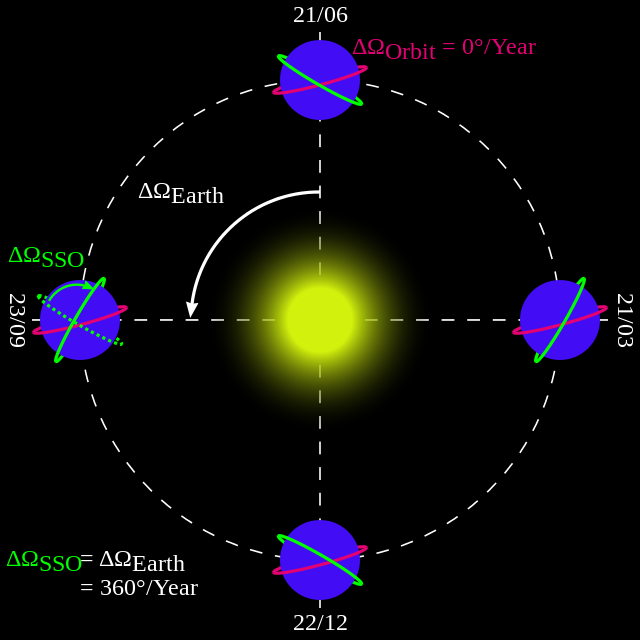
\includegraphics[scale=0.4]{sso}
 \end{figure}
 \begin{itemize}
  \item Höhe und Inklination werden so kombiniert, dass ein Satellite aus Sicht der Sonne immer auf dem selben Orbit ist
  \item Höhe: 600-800 km
  \item Inklination: leicht retrograd ($\approx 98^\circ$)
  \item Umlaufdauer: 96-100min
 \end{itemize}

 \item Geostationary Orbit GEO
 \begin{itemize}
  \item kreisförmiger Orbit
  \item Höhe: 35.786km
  \item Umlaufdauer: 24h
  \item Wettersatelliten, Kommunikationssatelliten, Fernsehsatelliten
 \end{itemize}

\end{enumerate}

\noindent \f{Subsatellite Point} = intersection of the line between satellite and earth center with the earth's surface 
\noindent \f{Hohmann Transfer}
\begin{figure}[!ht]
 \centering
 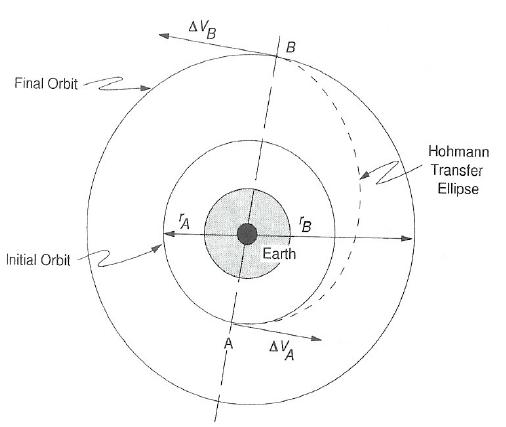
\includegraphics[scale=0.6]{hohmann}
\end{figure}

\begin{itemize}
\item Calculate a transfer between two circular orbits with radius $r_A$ to $r_B$. The velocity at pericenter of the transfer ellipse:
\[ v_P^2 = 2 \mu \left( \frac{1}{r_A} - \frac{1}{r_A + r_B} \right) = 2 \mu \frac{r_B}{r_A(r_A+r_B)} \]
\item The required $\Delta v_A$ to inject from the transfer orbit:
\[ \Delta v_A = v_P - v_A = \sqrt{\frac{\mu}{r_A}} \left( \sqrt{\frac{2r_B}{r_A+r_B}} -1\right) \]
\item The required $\Delta v$ to inject from the transfer orbit into orbit with $r_B$:
\[ \Delta v_B = v_B - v_\text{apo} = \sqrt{\frac{\mu}{r_B}} \left( 1 - \sqrt{\frac{2r_A}{r_A+r_B}}\right) \]
where $v_B$ is the circular velocity at $r_B$.
\item The Hohmann transfer is the most energy-efficient transfer between two circular orbits.
\[ \Delta v_\text{total} =  \Delta v_A + \Delta v_B = \sqrt{\mu}\left[ \sqrt{\left( \frac{2}{r_A} - \frac{2}{r_A+r_B} \right)} - \sqrt{\frac{1}{r_A}} + \sqrt{\frac{2}{r_B}-\frac{2}{r_A+r_B}} - \sqrt{\frac{1}{r_B}} \right]\]
\end{itemize}
